{\color{indiagreen}\subsection{Postavitev}}
V tem poglavju vam bom samo prikazal osnovno postavitev Unity urejevalnika in par njegovih funkcij.
\begin{figure}[ht!]
	\centering
	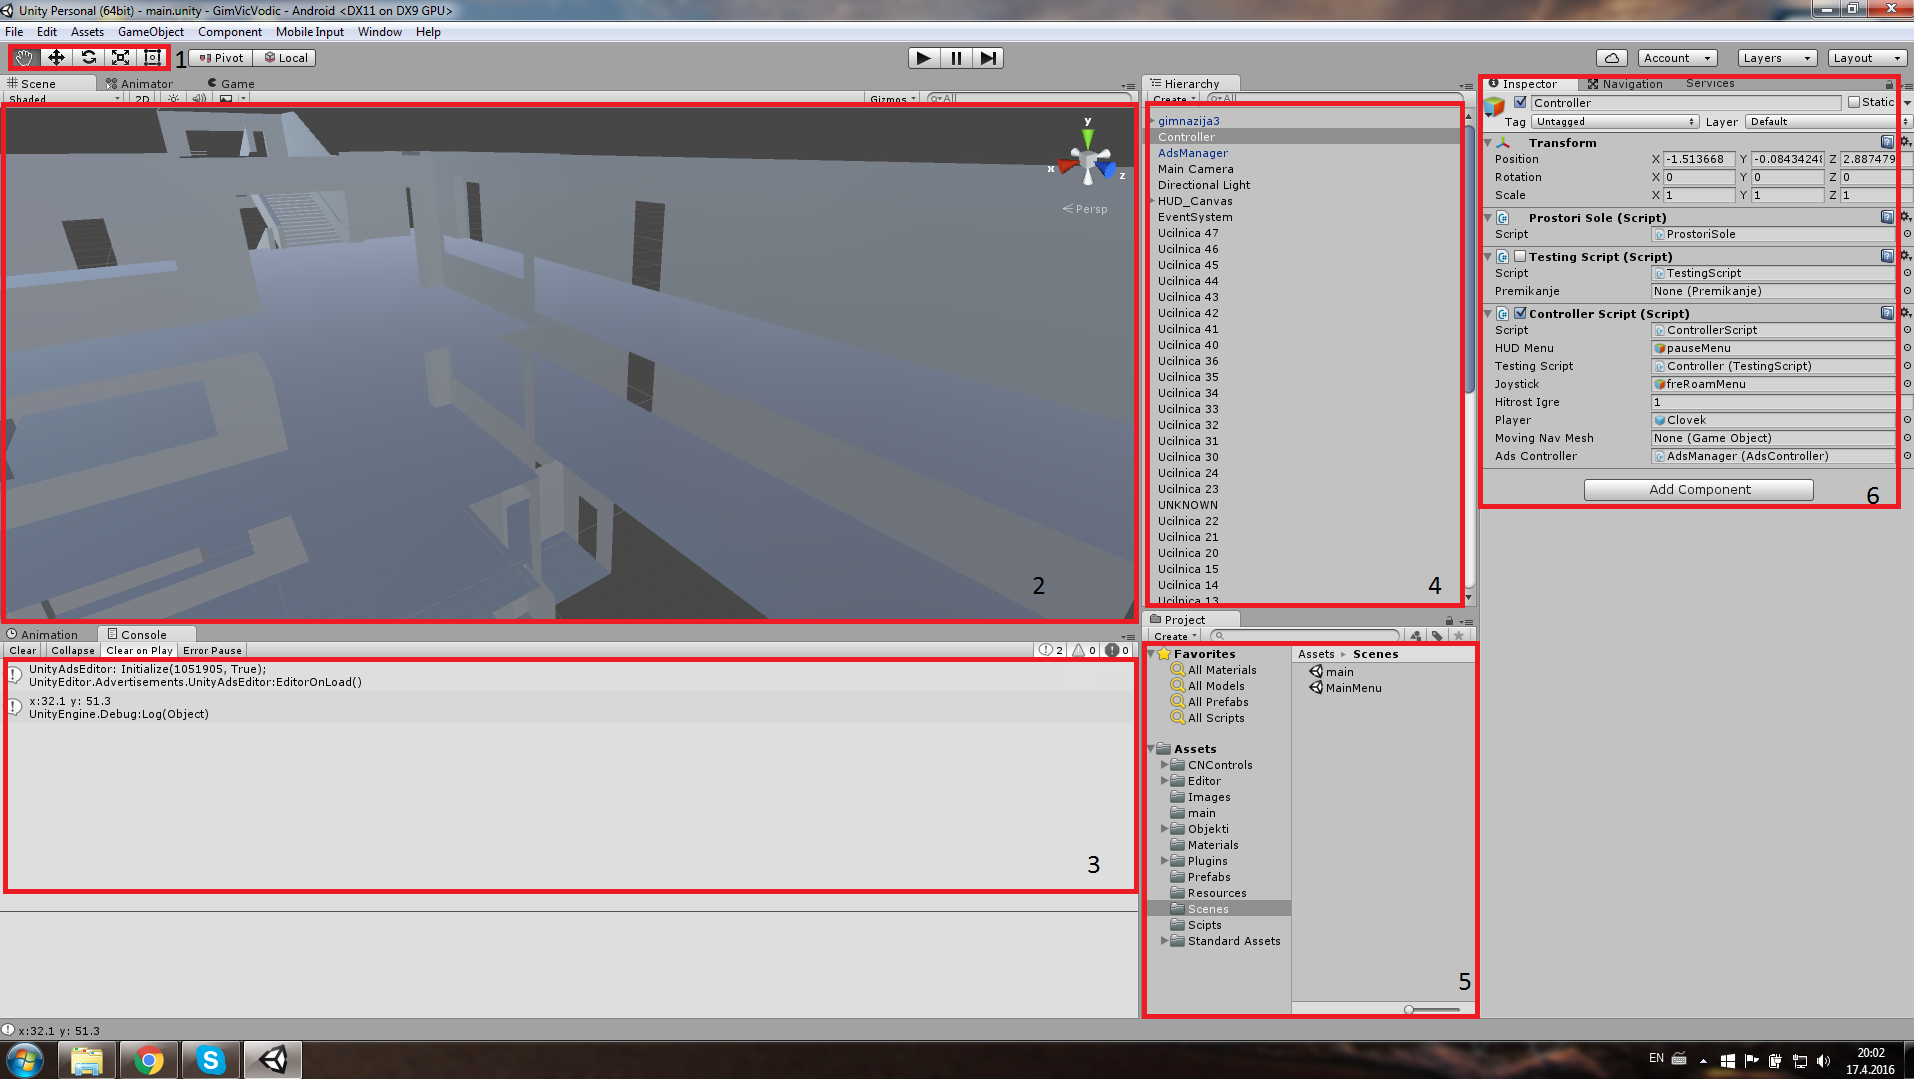
\includegraphics[width=16cm, height=12cm,keepaspectratio=true]{Postavitev1.png}
	\caption{Postavitev}
	{\tiny Vir: Osebni arhiv}
\end{figure}
\begin{enumerate}
	\item Bljižnice za spreminjanje orodja za delo z GameObject-i
	\item Pogled v sceno
	\item Kozola in njen izpis
	\item Hierarhija objektov in v objekti v njej
	\item Projektno drevo in datoteke
	\item Pregledovalnik trenutnega objekta
\end{enumerate}